\documentclass{article}
\usepackage[utf8]{inputenc}
\usepackage{tikz, pgfplots}
\usetikzlibrary{positioning}

\title{Tikz YouTube}
\author{Trefor Bazett}
\date{March 2022}

\begin{document}


\section{Tikz}




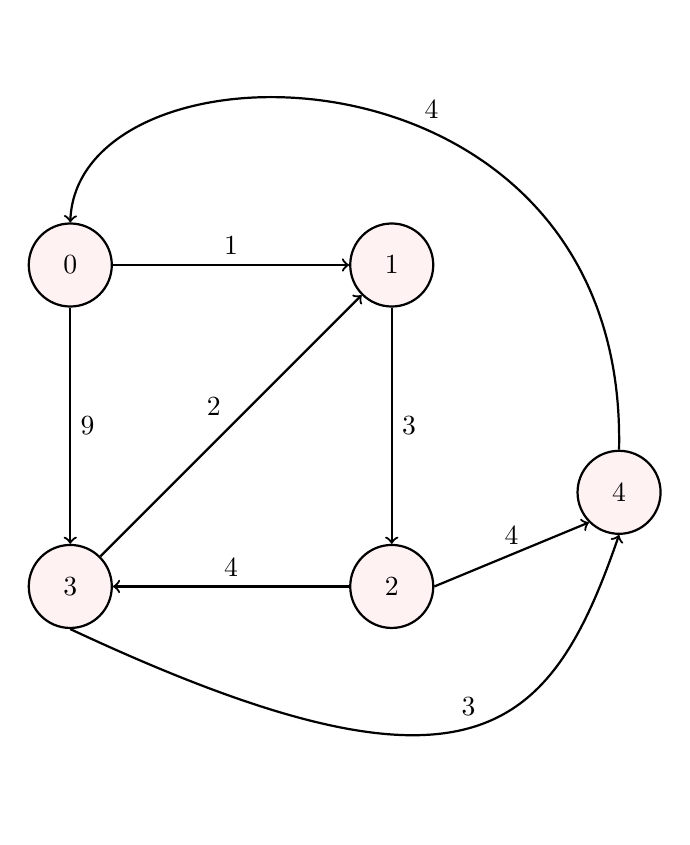
\begin{tikzpicture}[
city/.style={circle, draw=black, fill=red!5,  thick, minimum size=30},
oldnode/.style={rectangle, draw=blue!60, fill=blue!5, very thick, minimum size=40},
node distance=3cm
]
%Nodes
\node[city]        (C1)                            { $1$};
\node[city]        (C2)       [below=of C1]      { $2$};
%\node[city]        (RecO)       [below=of InfO]      { $R_O(t)$};

\node[city]      (C0)        [left=of C1]      { $0$};
\node[city]      (C3)        [left=of C2]      { $3$};
\node[city]      (C4)        [below right=of C1]      { $4$};


%Lines
\draw[->, thick] (C2.west) to node[above] {$4$} (C3.east) ;
\draw[->, thick] (C0.south) to node[right] {$9$} (C3.north) ;
\draw[->, thick] (C2.east) to node[above] {$4$} (C4.south west) ;
\draw[->, thick] (C1.south) to node[right] {$3$} (C2.north) ;
\draw[->, thick] (C0.east) to node[above] {$1$} (C1.west) ;
\draw[->, thick] (C3.north east) to node[above left] {$2$} (C1.south west) ;
\draw[->, thick] (C4.north) .. controls  (3,3) and (-4,3)   .. (C0.north)node[black, above=1pt,pos=0.4]{$4$};
\draw[->, thick] (C3.south) .. controls  (1,-7) and (2,-6)   .. (C4.south)
node[black, above=1pt,pos=0.5]{$3$};;
\end{tikzpicture}

\vspace{10px}

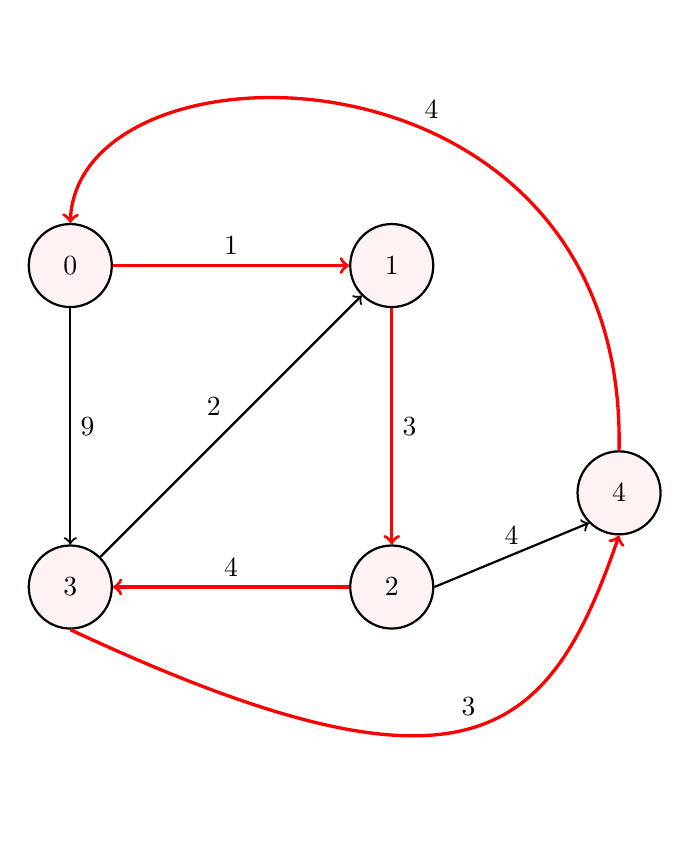
\begin{tikzpicture}[
city/.style={circle, draw=black, fill=red!5,  thick, minimum size=30},
oldnode/.style={rectangle, draw=blue!60, fill=blue!5, very thick, minimum size=40},
node distance=3cm
]
%Nodes
\node[city]        (C1)                            { $1$};
\node[city]        (C2)       [below=of C1]      { $2$};
%\node[city]        (RecO)       [below=of InfO]      { $R_O(t)$};

\node[city]      (C0)        [left=of C1]      { $0$};
\node[city]      (C3)        [left=of C2]      { $3$};
\node[city]      (C4)        [below right=of C1]      { $4$};


%Lines
\draw[->, very thick,red] (C2.west) to node[above,black] {$4$} (C3.east) ;
\draw[->, thick] (C0.south) to node[right,black] {$9$} (C3.north) ;
\draw[->, thick] (C2.east) to node[above] {$4$} (C4.south west) ;
\draw[->, very thick, red] (C1.south) to node[right, black] {$3$} (C2.north) ;
\draw[->, very thick, red] (C0.east) to node[above, black] {$1$} (C1.west) ;
\draw[->, thick] (C3.north east) to node[above left] {$2$} (C1.south west) ;
\draw[->, very thick, red] (C4.north) .. controls  (3,3) and (-4,3)   .. (C0.north)node[black, above=1pt,pos=0.4]{$4$};
\draw[->, very thick,red] (C3.south) .. controls  (1,-7) and (2,-6)  .. (C4.south) node[black, above=1pt,pos=0.5]{$3$};
\end{tikzpicture}

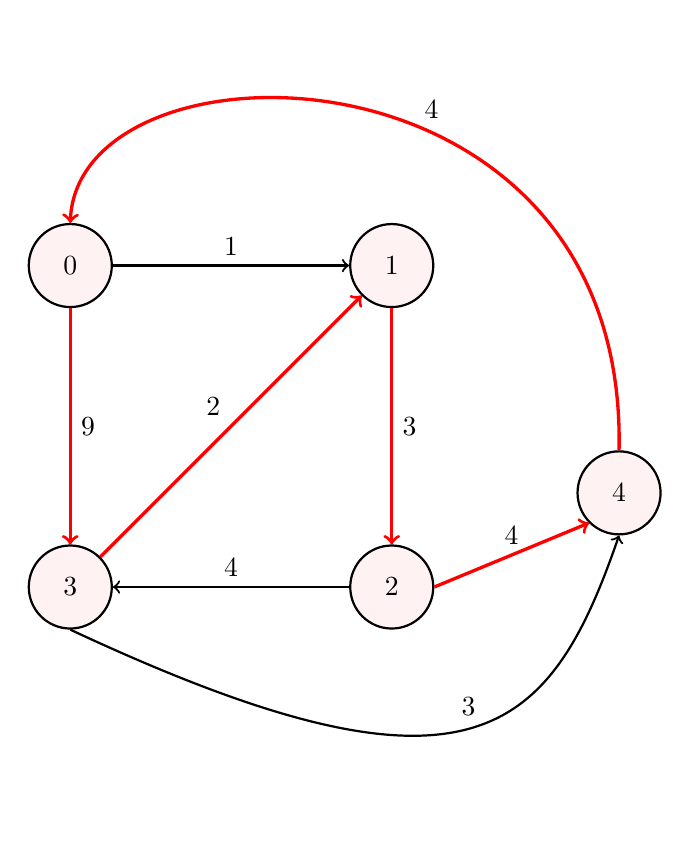
\begin{tikzpicture}[
city/.style={circle, draw=black, fill=red!5,  thick, minimum size=30},
oldnode/.style={rectangle, draw=blue!60, fill=blue!5, very thick, minimum size=40},
node distance=3cm
]
%Nodes
\node[city]        (C1)                            { $1$};
\node[city]        (C2)       [below=of C1]      { $2$};
%\node[city]        (RecO)       [below=of InfO]      { $R_O(t)$};

\node[city]      (C0)        [left=of C1]      { $0$};
\node[city]      (C3)        [left=of C2]      { $3$};
\node[city]      (C4)        [below right=of C1]      { $4$};


%Lines
\draw[->, thick] (C2.west) to node[above,black] {$4$} (C3.east) ;
\draw[->, very thick,red] (C0.south) to node[right,black] {$9$} (C3.north) ;
\draw[->, very thick,red] (C2.east) to node[above,black] {$4$} (C4.south west) ;
\draw[->, very thick, red] (C1.south) to node[right, black] {$3$} (C2.north) ;
\draw[->, thick] (C0.east) to node[above, black] {$1$} (C1.west) ;
\draw[->, very thick,red] (C3.north east) to node[above left, black] {$2$} (C1.south west) ;
\draw[->, very thick, red] (C4.north) .. controls  (3,3) and (-4,3)   .. (C0.north)node[black, above=1pt,pos=0.4]{$4$};
\draw[->, thick] (C3.south) .. controls  (1,-7) and (2,-6)  .. (C4.south) node[black, above=1pt,pos=0.5]{$3$};
\end{tikzpicture}


\end{document}
